%----------------------------------------------------%
%           Written by Gaurav Gupta                  %
%    SC21B026, Aerospace Engineering (2021 Batch)    %
%       Inspired by the CALTECH Beamer Theme         %
%----------------------------------------------------%

\documentclass[hyperref={bookmarks=false},aspectratio=169]{beamer}
\usepackage[utf8]{inputenc}

%-------------------------Packages------------------------
\usepackage[utf8]{inputenc}
\usepackage{subcaption}
\usepackage{amsmath}
%---------------------------------------------------------
% -----------Define theme and color scheme----------------

\usetheme[sidebarleft]{IIST}  % 3 options: minimal, sidebarleft, sidebarright

% ---------Information on the title page------------------
	% ---------Information on the title page------------------
\title[Präsentation des Projekts]
{\bfseries{Präsentation des Projekts\\
	Für den Block\\
	Praxisorientiertes Programmierprojekt in Java (App)\\
	 (PhileTipTip / Philetairus Admin Tool)}}

\author[Matthias Christian Hochmuth]
{Matthias Christian Hochmuth}

\date{07.11.2024}
%------------------------------------------------------------

%------------------------------------------------------------

%------------------------------------------------------------
%The next block of commands puts the table of contents at the beginning of each section and highlights the current section:

% \AtBeginSection[]
% {
%   \begin{frame}
%     \frametitle{Table of Contents}
%     \tableofcontents[currentsection]
%   \end{frame}
% }
%------------------------------------------------------------

\begin{document}

\frame{\titlepage}  % Creates title page

%--------table of contents after title page---------------
\begin{frame}
\frametitle{Agenda}
\tableofcontents
\end{frame}
%---------------------------------------------------------

\section{Einleitung}
	\begin{frame}
  \frametitle{Problemstellung}

  \begin{alertblock}{Aktuelle Probleme der Philetairus Immobilien GmbH}
 	\begin{itemize}
	\item Nachholbedarf im Bereich der Digitalisierung
	 \item zunehmende Technikaffinität der Mieter
	\item Viele interne Prozesse nicht mehr zeitgemäß, schwerfällig und unflexibel
	\end{itemize}
  \end{alertblock}
\end{frame}
	\begin{frame}
  \frametitle{Lösungsansatz}

  \begin{block}{Lösungsansatz für die Probleme der Philetairus Immobilien GmbH}
 	\begin{itemize}
	\item Informationstechnologie Abteilung erheblich ausbauen
	 \item Transformation der IT-Abteilung - Schaffung einer Entwicklungsabteilung
	\item Teilbereich des Unternehmens digitalisieren um Erfahrungen zu sammeln
	\item Agile Prozesse einführen um flexibel zu bleiben
	\item  Pilotprojekt PhileTipTip - App zur Meldung von Schäden an Grünanlagen
	\end{itemize}
  \end{block}
\end{frame}

%---------------------------------------------------------

\section{Vorbereitung}
	\begin{frame}
\frametitle{Geschäftsprozessmodellierung}

\begin{figure}
  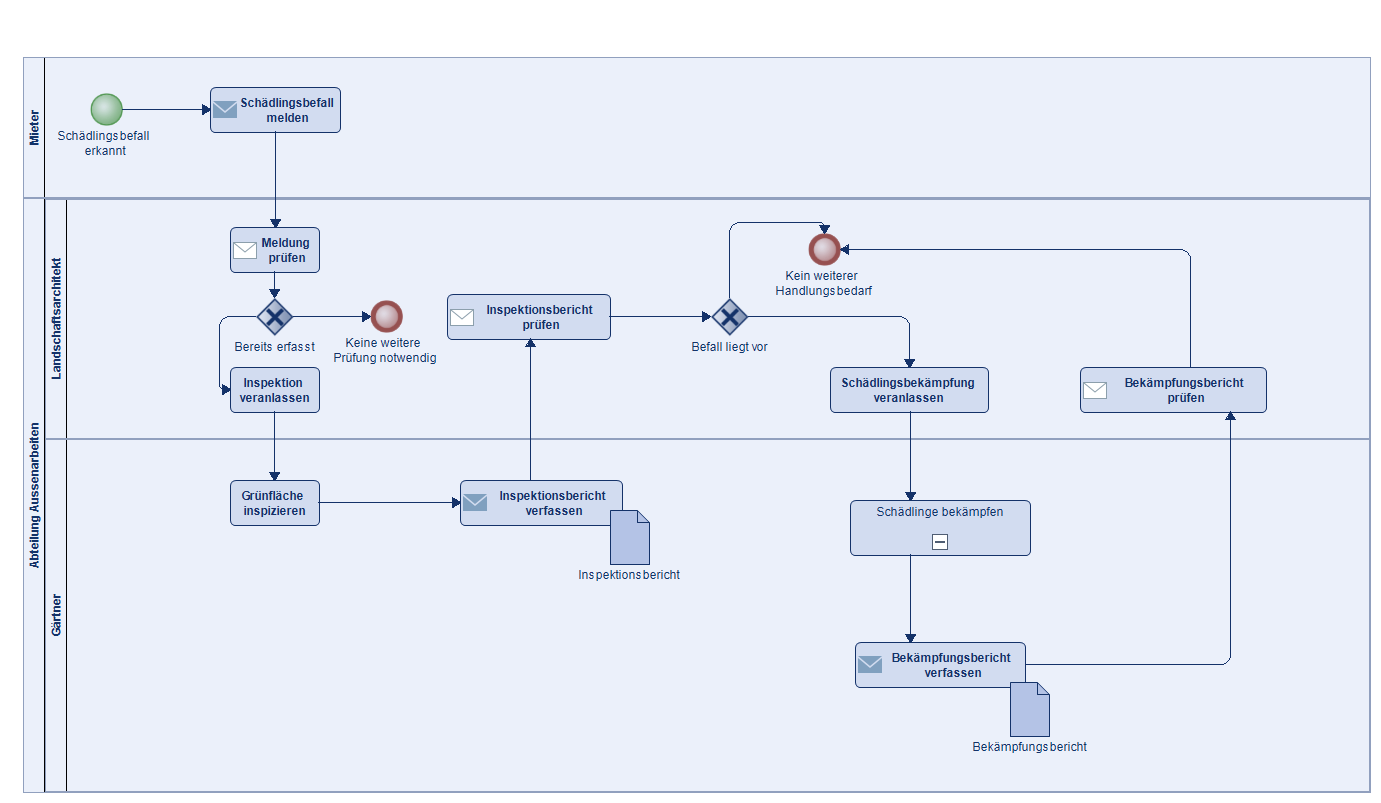
\includegraphics[width=0.8\textwidth]{figures/BPM.png}
  \label{fig:BPM}
\end{figure}

\end{frame}





	\begin{frame}
  \frametitle{Anforderungsanalyse}

  \begin{block}{ Funktionale Anforderungen}
 	\begin{itemize}
	\item Erfassung von Meldungen über Schädlingsbefall
	 \item Speichern der Meldungen
	\item Anzeige und Sortierung dieser Meldungen
	\end{itemize}
  \end{block}

  \begin{alertblock}{Nichtfunktionale Anforderungen}
 	\begin{itemize}
	\item Daten On-Premises (auf Firmeninterner Hardware)
	 \item Einfache Bedienbarkeit der App
	\item Leichte Wartbarkeit der App
	\item Leichte Erweiterbarkeit der App
	\end{itemize}
  \end{alertblock}

\end{frame}
	\begin{frame}
  \frametitle{User Stories (Auszug)}

  \begin{table}
    \centering
    \begin{tabular}{||c|c|c||}
      \hline
      \textbf{Als [Rolle]} & \textbf{möchte ich [Funktionalität]} & \textbf{damit [Grund]}\\
      \hline
      Mieter & Unkrautbewuchs melden & die Gärtner ihn beseitigen \\
      \hline
      Teamleiter & Meldungen ans Team senden & Arbeiten zu koordinieren \\
      \hline
      Gärtner &  sehen, wo ich arbeiten soll & den Einsatzort schnell finde \\
      \hline
      Abteilungsleiter &  Meldungen einsehen können & evtl. Muster zu erkennen \\
      \hline
    \end{tabular}
  \end{table}
\end{frame}

	
%---------------------------------------------------------

\section{Umsetzung}
	%Changing visivility of the text
\begin{frame}
\frametitle{Vorgehen und Techstack}
	Für die Umsetzung wurde der folgendes Vorgehen und folgender Techstack beschlossen:

	\begin{itemize}
		\item inkrementelle und iterative Entwicklung
		\item Jira für die Koordination und das Projektmanagement
		\item Entwicklung mit Java nach OOP Prinzipien
		\item Einsatz von Patterns, SOLID Prinzipien, Frameworks etc. 
		\item Android Studio für die App, IntelliJ für das Admin Tool
		\item Git für die Versionsverwaltung, CI/CD
	\end{itemize}
\end{frame}
	\begin{frame}
\frametitle{Iterative und Inkrementelle Entwicklung}

\begin{figure}
  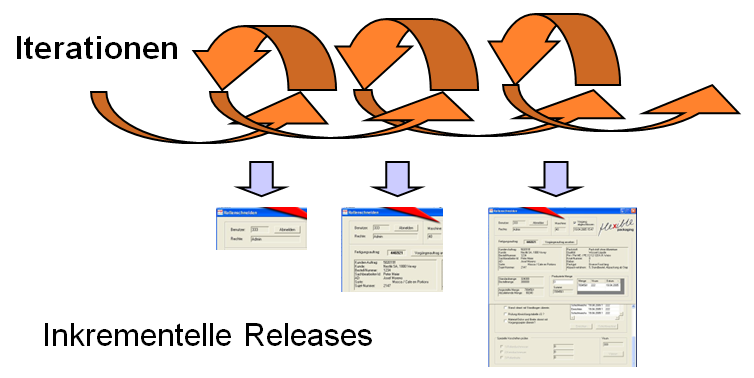
\includegraphics[width=0.7\textwidth]{figures/softwarecity_iterativ.png}
  \label{fig:iterativ}
\end{figure}

\end{frame}





	\begin{frame}
\frametitle{Jira}

\begin{figure}
  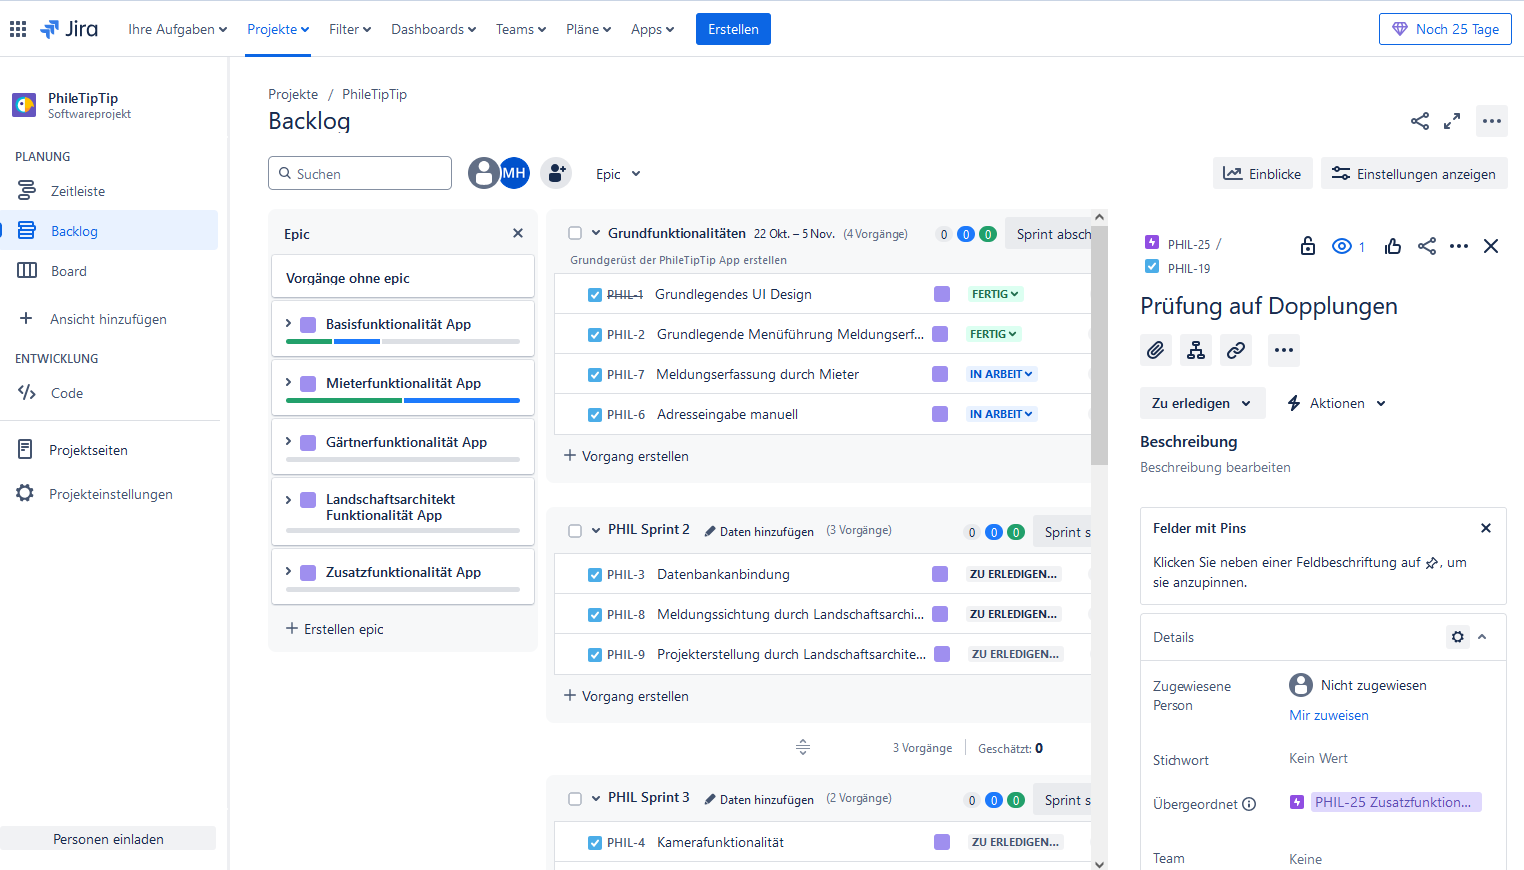
\includegraphics[width=0.8\textwidth]{figures/Jira.png}
  \label{fig:jira}
\end{figure}

\end{frame}





	\begin{frame}
\frametitle{Git GUI}

\begin{figure}
  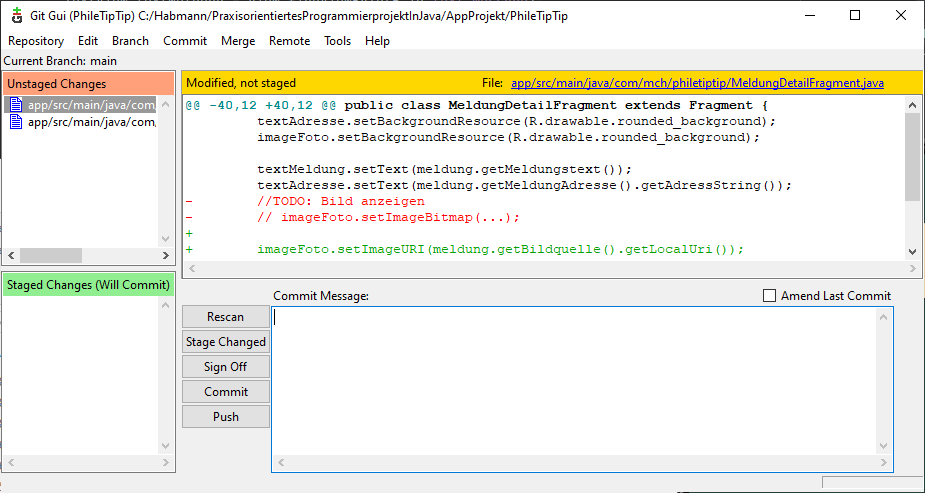
\includegraphics[width=0.8\textwidth]{figures/gitgui.png}
  \caption{Git Gui}
  \label{fig:gitgui}
\end{figure}

\end{frame}





	\begin{frame}
\frametitle{Component Diagram}

\begin{figure}
  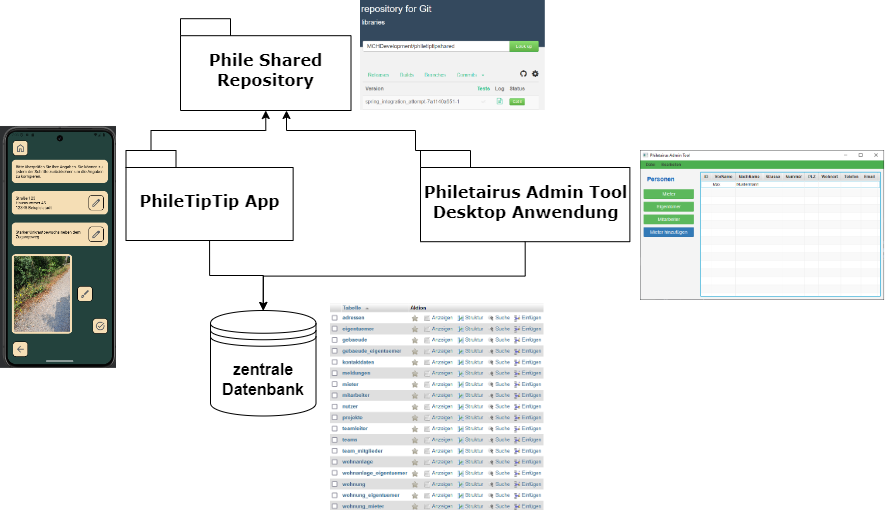
\includegraphics[width=0.8\textwidth]{figures/Component_Diagramm.drawio.png}
  \label{fig:component}
\end{figure}

\end{frame}





	\begin{frame}
\frametitle{Class Diagram}

\begin{figure}
  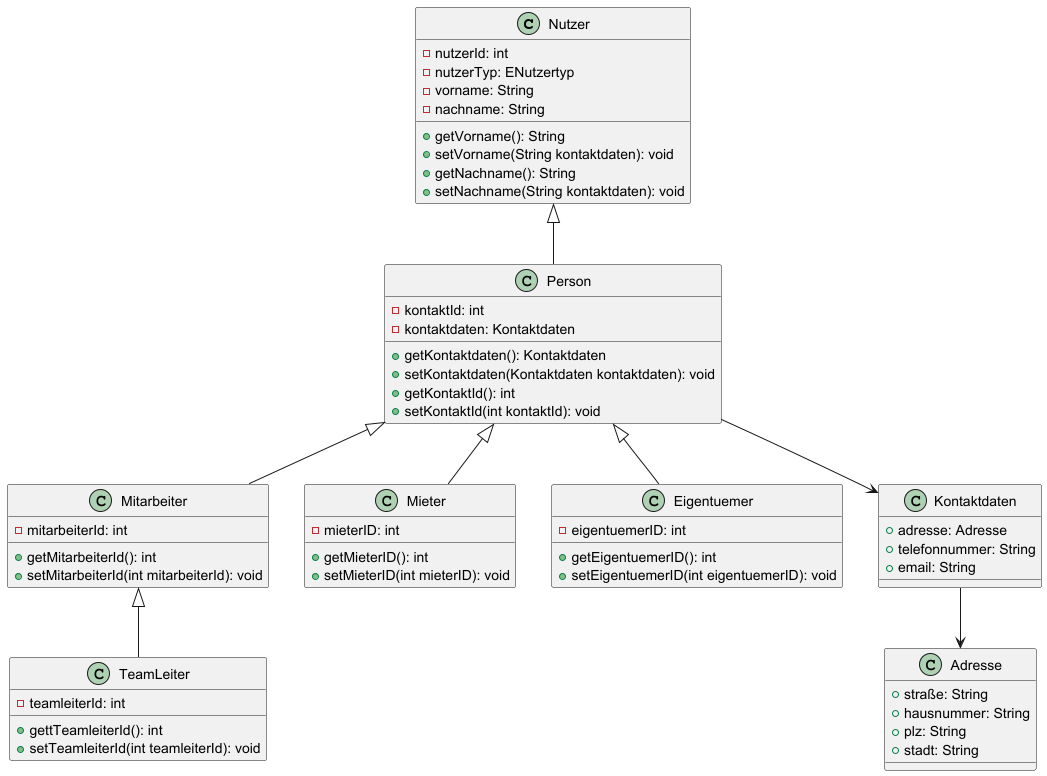
\includegraphics[height=0.9\textheight]{figures/model_Person.png}
  \caption{Class Diagram}
  \label{fig:class}
\end{figure}

\end{frame}






%---------------------------------------------------------

\section{Resultat und Präsentation}
	\begin{frame}
\frametitle{PhileTipTip}

\begin{figure}
  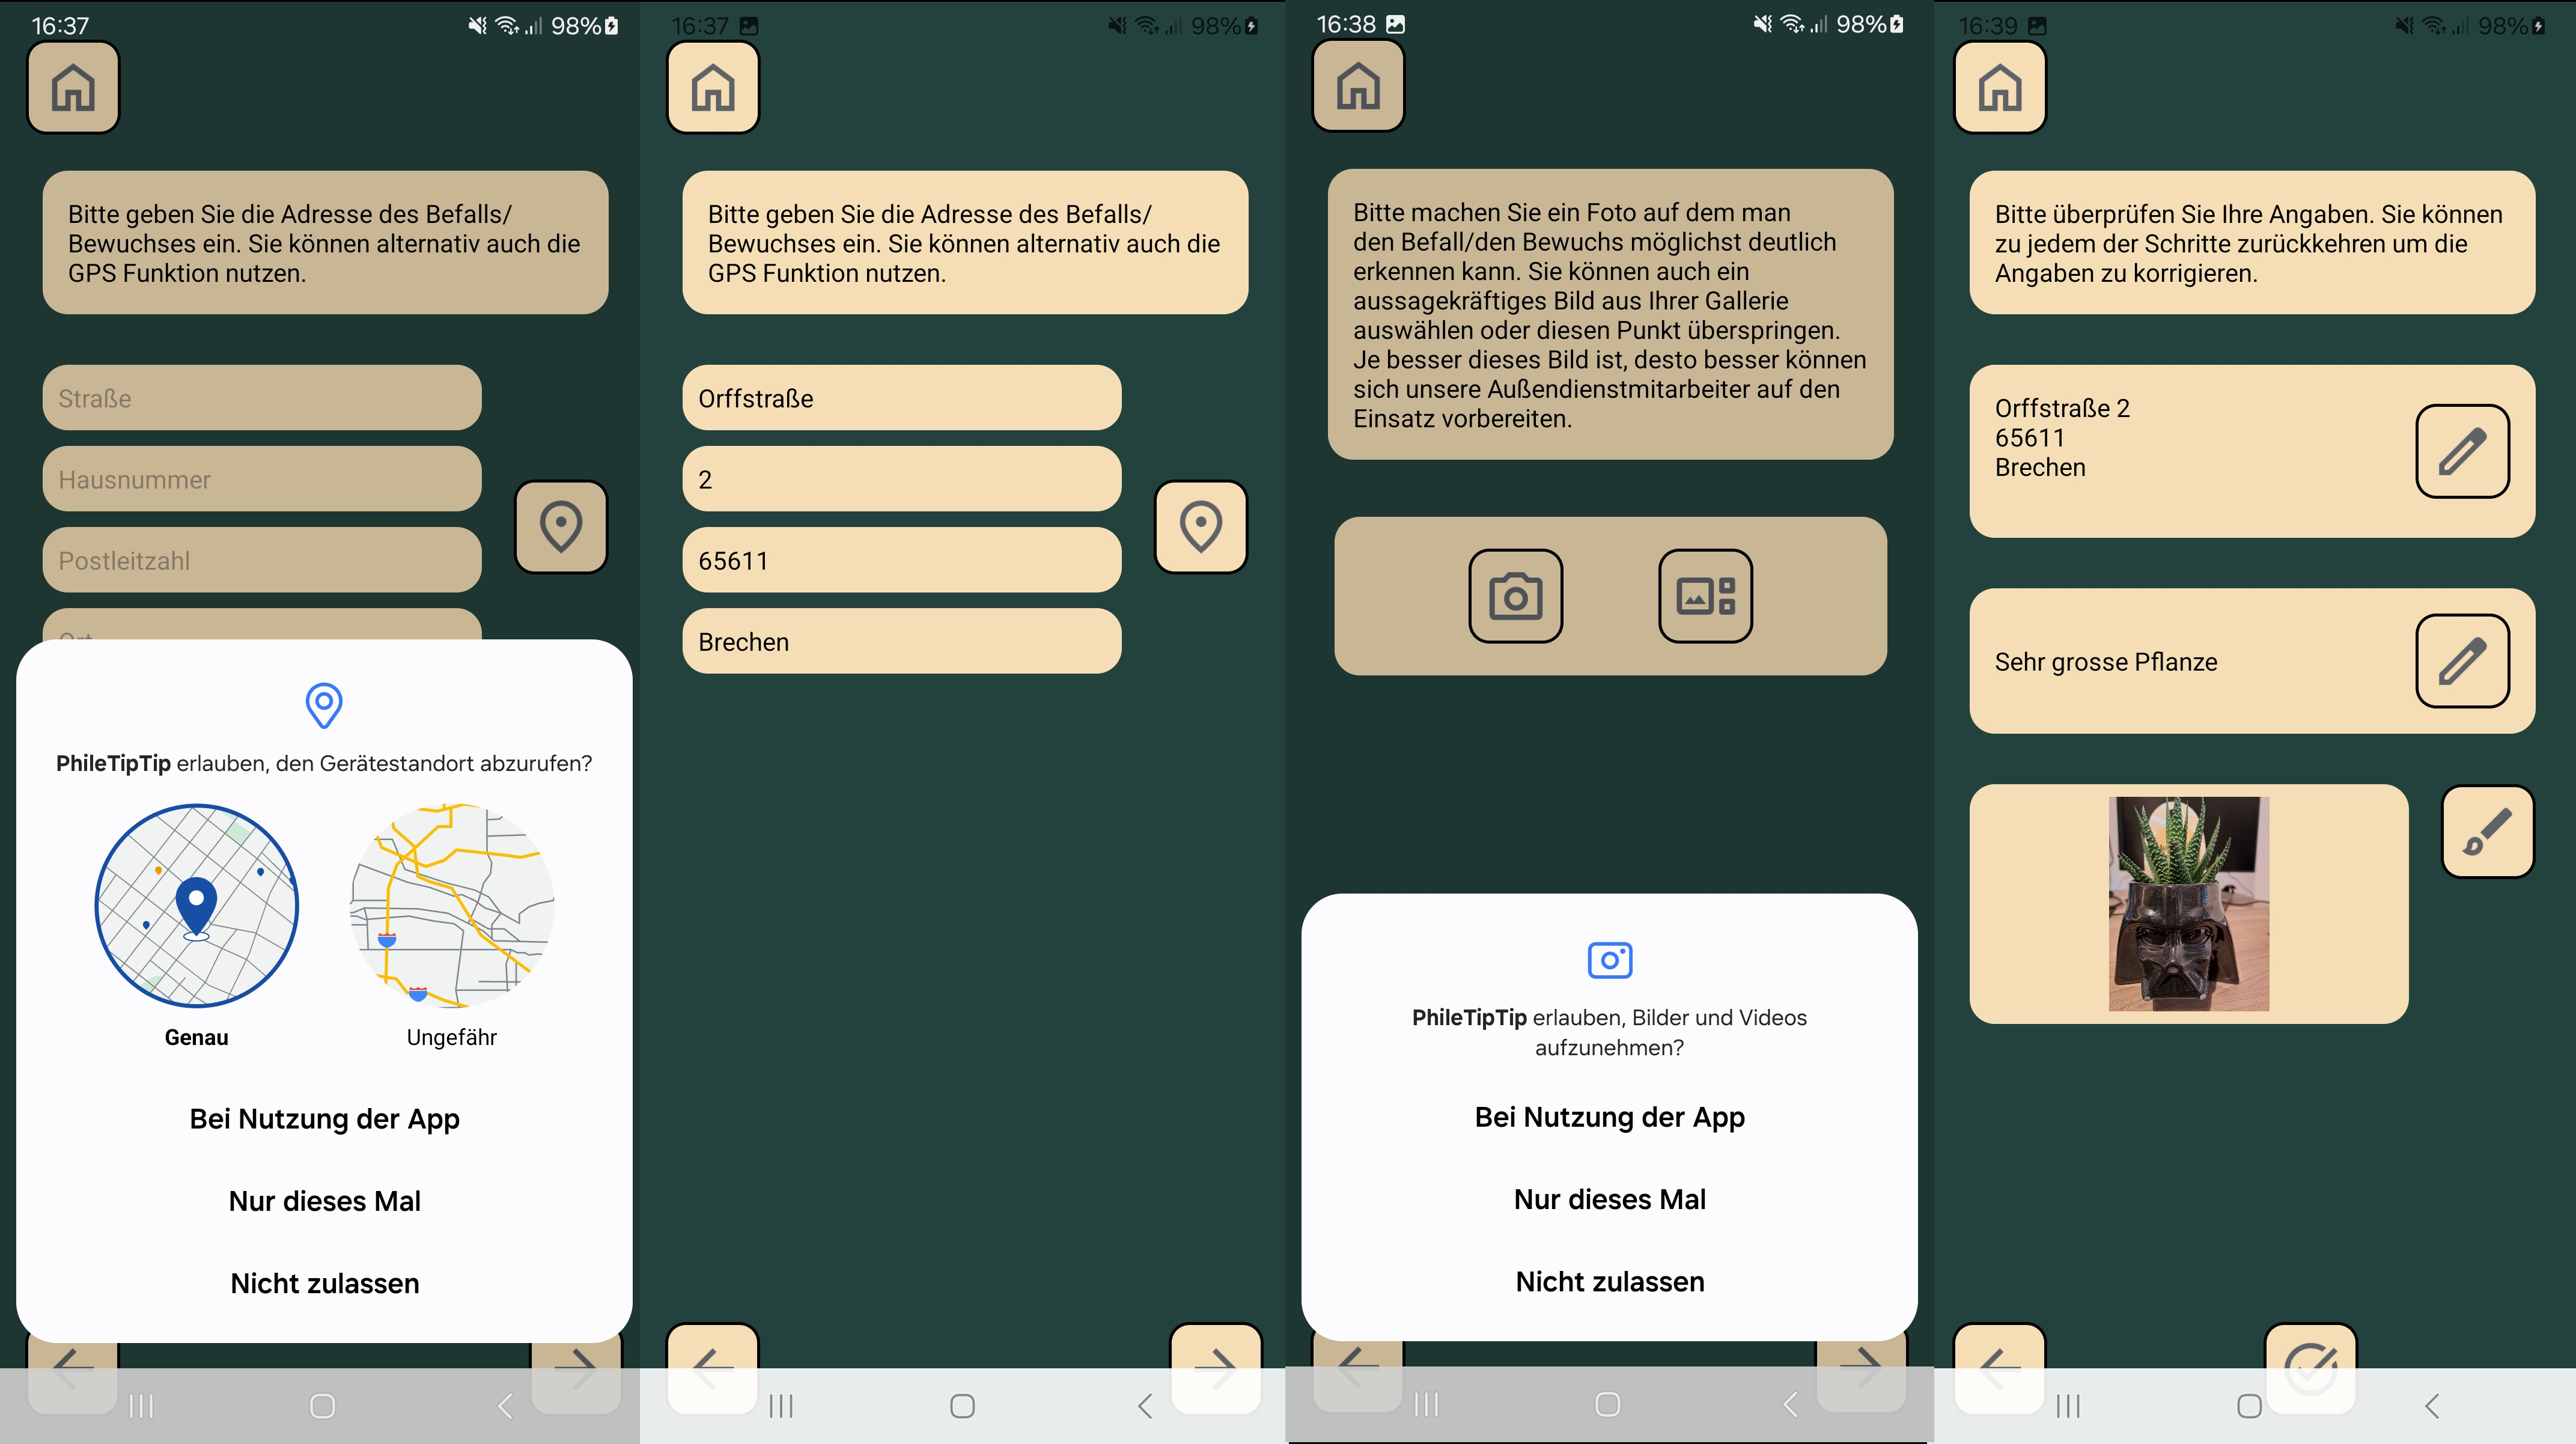
\includegraphics[width=0.8\textwidth]{figures/userworkflow.jpg}
  \caption{User Workflow}
  \label{fig:workflow}
\end{figure}

\end{frame}





	\begin{frame}
\frametitle{Philetairus Admin Tool}

\begin{figure}
  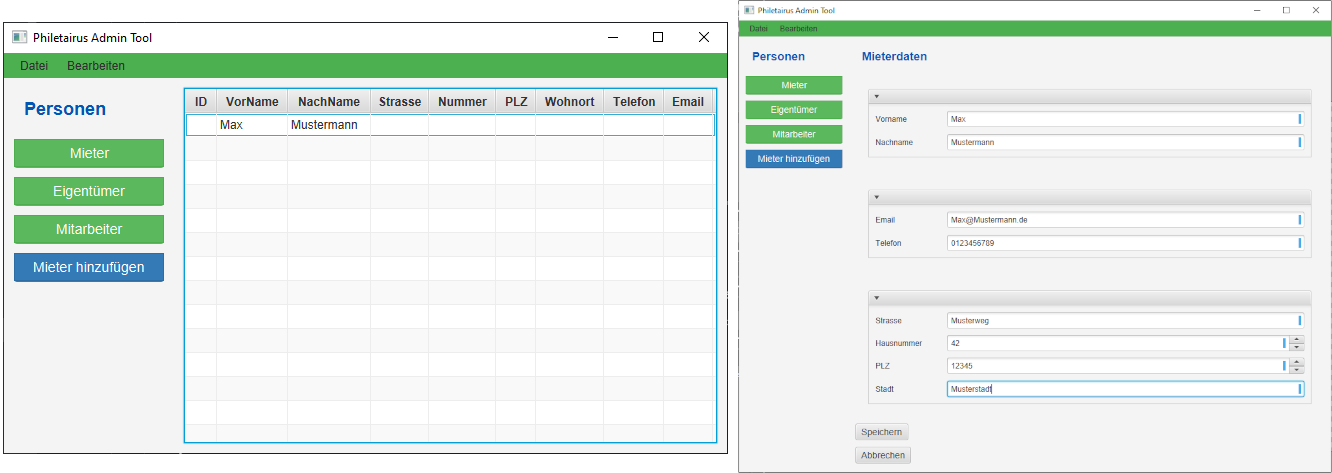
\includegraphics[width=0.8\textwidth]{figures/phileadmin_workflow.png}
  \label{fig:phileadmin}
\end{figure}

\end{frame}





	%Changing visivility of the text
\begin{frame}
\frametitle{Kurze Präsentation der Funktionalität}
	PhileTipTip App ind Philetairus Admin Tool

\end{frame}

%---------------------------------------------------------

\section{Finale}
	\begin{frame}
  \frametitle{Ausblick}

  \begin{block}{Nächste Schritte}
 	\begin{itemize}
	\item Weiterentwicklung Admin Tool
	 \item Grafische Verbesserungen PhileTipTip
	\item Gärtnerfunktionalitäten PhileTipTip (Einsatzanweisungen)
	\end{itemize}
  \end{block}

  \begin{alertblock}{Mögliche Folgeprojekte}
 	\begin{itemize}
	\item Digitalisierung weiterer Abteilungen (Haustechnik, Hausreinigung)
	 \item Automatisierung von Prozessen
	\item Schnittstellen zu anderen Systemen (Stadtwerke, Finanzamt)
	\end{itemize}
  \end{alertblock}

\end{frame}
	\begin{frame}
\frametitle{Ende}

\begin{columns}

\column{0.6\textwidth}
\begin{itemize}
\item Dieser Vortrag ist zu Ende
\item Die Digitalisierung hat gerade erst Begonnen
\end{itemize}

\column{0.4\textwidth}
\begin{figure}
  
\includegraphics[width=0.8\textwidth]{figures/loading.png}
  \label{fig:prince}
\end{figure}
\end{columns}

\end{frame}






\end{document}